\documentclass{article}

\usepackage{amsmath}
\usepackage{amssymb}
\usepackage{amsthm}
\usepackage[australian]{babel}
\usepackage{braket}
\usepackage[a4paper]{geometry}
\usepackage{tikz}

%\usetikzlibrary{external}
%\tikzexternalize[prefix=tikz/]

\usetikzlibrary{shapes.geometric}
\usetikzlibrary{shapes.misc}
% Base style for tensors.
\tikzstyle{tensor}=[draw, inner sep=0pt, minimum size=10pt]
% Used for drawing gaps in the tensor network diagram.
\tikzstyle{notensor}=[minimum size=10pt]
% Style for A tensors: if a square-shaped node is desired instead, ‘circle’ can be removed here.
\tikzstyle{atensor}=[tensor, circle]
% Circular-style tensors, for regular matrices.
\tikzstyle{ctensor}=[tensor, circle]
% Diamond-style tensors, for diagonal matrices.
\tikzstyle{dtensor}=[tensor, diamond]
% MPO tensors.
\tikzstyle{wtensor}=[tensor]
% Left-/right-orthogonal tensors.
% Triangular style (unused).
% Drawing left-/right-orthogonal tensors as isosceles triangles results in an
% undesirable alignment, so we draw them as trapezia instead where one of the
% parallel edges has zero length.
% (For some reason, inner xsep=0pt produces an error here, so we just use 0.001pt.)
%\tikzstyle{ltensor}=[tensor, isosceles triangle, shape border rotate=0, isosceles triangle apex angle=60]
%\tikzstyle{rtensor}=[tensor, isosceles triangle, shape border rotate=180, isosceles triangle apex angle=60]
%\tikzstyle{ltensor}=[tensor, trapezium, shape border rotate=270, trapezium stretches, minimum width=20pt/sqrt(3), minimum height=10pt, inner xsep=0.001pt, shape border rotate=270]
%\tikzstyle{rtensor}=[tensor, trapezium, shape border rotate=270, trapezium stretches, minimum width=20pt/sqrt(3), minimum height=10pt, inner xsep=0.001pt, shape border rotate=90]
% Rounded circle style.
\tikzstyle{ltensor}=[tensor, rounded rectangle, rounded rectangle left arc=none]
\tikzstyle{rtensor}=[tensor, rounded rectangle, rounded rectangle right arc=none]
% Environment (E/F) tensors.
\tikzstyle{etensor}=[tensor, minimum height=38.5pt]

\title{Ti\textit{k}Z tensor network diagrams}
\author{Jesse Osborne}

\begin{document}
\maketitle

\noindent
Finite MPS:
\begin{equation}
    \ket{\Psi} =
    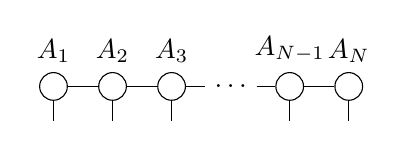
\begin{tikzpicture}[baseline=-0.25em]
        \node[atensor, label=\(A_1\)]     (A1) at (0, 0) {};
        \node[atensor, label=\(A_2\)]     (A2) at (0.75, 0) {};
        \node[atensor, label=\(A_3\)]     (A3) at (1.5, 0) {};
        \node[notensor]                   (A4) at (2.25, 0) {\(\ldots\)};
        \node[atensor, label=\(A_{N-1}\)] (A5) at (3, 0) {};
        \node[atensor, label=\(A_N\)]     (A6) at (3.75, 0) {};
        \draw (A1.south) -- +(0, -0.25);
        \draw (A2.south) -- +(0, -0.25);
        \draw (A3.south) -- +(0, -0.25);
        \draw (A5.south) -- +(0, -0.25);
        \draw (A6.south) -- +(0, -0.25);
        \draw (A1) -- (A2) -- (A3) -- (A4) -- (A5) -- (A6);
    \end{tikzpicture}
    .
\end{equation}
Gauge transform:
\begin{equation}
    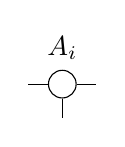
\begin{tikzpicture}[baseline=-0.25em]
        \node[atensor, label=\(A_i\)] (A1) at (1, 0) {};
        \draw (A1.south) -- +(0, -0.25);
        \draw (A1.west) -- +(-0.25, 0);
        \draw (A1.east) -- +(0.25, 0);
    \end{tikzpicture}
    \rightarrow
    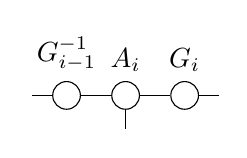
\begin{tikzpicture}[baseline=-0.25em]
        \node[ctensor, label=\(G_{i-1}^{-1}\)] (G0inv) at (0.25, 0) {};
        \node[atensor, label=\(A_i\)] (A1) at (1, 0) {};
        \node[ctensor, label=\(G_i\)] (G1) at (1.75, 0) {};
        \draw (A1.south) -- +(0, -0.25);
        \draw (G0inv.west) -- +(-0.25, 0);
        \draw (G1.east) -- +(0.25, 0);
        \draw (G0inv) -- (A1) -- (G1);
    \end{tikzpicture}
    .
\end{equation}
Left-orthogonal form:
\begin{equation}
    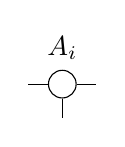
\begin{tikzpicture}[baseline=-0.25em]
        \node[atensor, label=\(A_i\)] (A1) at (1, 0) {};
        \draw (A1.south) -- +(0, -0.25);
        \draw (A1.west) -- +(-0.25, 0);
        \draw (A1.east) -- +(0.25, 0);
    \end{tikzpicture}
    \rightarrow
    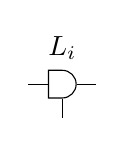
\begin{tikzpicture}[baseline=-0.25em]
        \node[ltensor, label=\(L_i\)] (A1) at (1, 0) {};
        \draw (A1.south) -- +(0, -0.25);
        \draw (A1.west) -- +(-0.25, 0);
        \draw (A1.east) -- +(0.25, 0);
    \end{tikzpicture}
    ,
    \qquad
    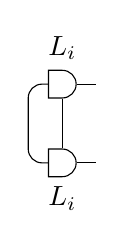
\begin{tikzpicture}[baseline=-0.25em]
        \node[ltensor, label=\(L_i\)] (A1) at (1, 0.5) {};
        \node[ltensor, label=below:\(L_i\)] (A1conj) at (1, -0.5) {};
        \draw (A1.south) -- (A1conj.north);
        \draw[rounded corners=5pt] (A1.west) -- +(-0.25, 0) -- +(-0.25, -1) -- (A1conj.west);
        \draw (A1.east) -- +(0.25, 0);
        \draw (A1conj.east) -- +(0.25, 0);
    \end{tikzpicture}
    =
    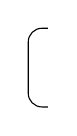
\begin{tikzpicture}[baseline=-0.25em]
        \draw[rounded corners=5pt] (0, 0.5) -- +(-0.25, 0) -- +(-0.25, -1) -- +(0, -1);
    \end{tikzpicture}
    .
\end{equation}
Right-orthogonal form:
\begin{equation}
    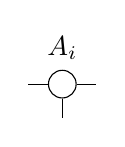
\begin{tikzpicture}[baseline=-0.25em]
        \node[atensor, label=\(A_i\)] (A1) at (1, 0) {};
        \draw (A1.south) -- +(0, -0.25);
        \draw (A1.west) -- +(-0.25, 0);
        \draw (A1.east) -- +(0.25, 0);
    \end{tikzpicture}
    \rightarrow
    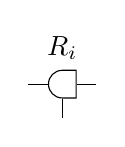
\begin{tikzpicture}[baseline=-0.25em]
        \node[rtensor, label=\(R_i\)] (A1) at (1, 0) {};
        \draw (A1.south) -- +(0, -0.25);
        \draw (A1.west) -- +(-0.25, 0);
        \draw (A1.east) -- +(0.25, 0);
    \end{tikzpicture}
    ,
    \qquad
    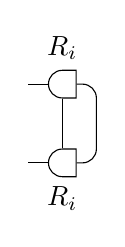
\begin{tikzpicture}[baseline=-0.25em]
        \node[rtensor, label=\(R_i\)] (A1) at (1, 0.5) {};
        \node[rtensor, label=below:\(R_i\)] (A1conj) at (1, -0.5) {};
        \draw (A1.south) -- (A1conj.north);
        \draw[rounded corners=5pt] (A1.east) -- +(0.25, 0) -- +(0.25, -1) -- (A1conj.east);
        \draw (A1.west) -- +(-0.25, 0);
        \draw (A1conj.west) -- +(-0.25, 0);
    \end{tikzpicture}
    =
    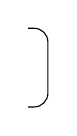
\begin{tikzpicture}[baseline=-0.25em]
        \draw[rounded corners=5pt] (0, 0.5) -- +(0.25, 0) -- +(0.25, -1) -- +(0, -1);
    \end{tikzpicture}
    .
\end{equation}
SVD:
\begin{equation}
    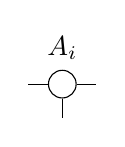
\begin{tikzpicture}[baseline=-0.25em]
        \node[atensor, label=\(A_i\)] (A1) at (1, 0) {};
        \draw (A1.south) -- +(0, -0.25);
        \draw (A1.west) -- +(-0.25, 0);
        \draw (A1.east) -- +(0.25, 0);
    \end{tikzpicture}
    =
    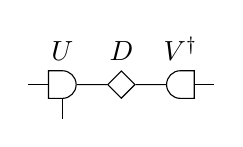
\begin{tikzpicture}[baseline=-0.25em]
        \node[ltensor, label=\(U\)] (A1) at (0.25, 0) {};
        \node[dtensor, label=\(D\)] (D) at (1, 0) {};
        \node[rtensor, label=\(V^\dag\)] (Vdag) at (1.75, 0) {};
        \draw (A1.south) -- +(0, -0.25);
        \draw (A1.west) -- +(-0.25, 0);
        \draw (Vdag.east) -- +(0.25, 0);
        \draw (A1) -- (D) -- (Vdag);
    \end{tikzpicture}
    .
\end{equation}
Mixed-canonical form:
\begin{equation}
    \ket{\Psi} =
    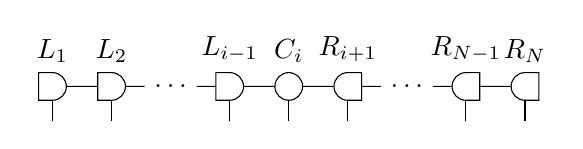
\begin{tikzpicture}[baseline=-0.25em]
        \node[ltensor, label=\(L_1\)]     (A1) at (0, 0) {};
        \node[ltensor, label=\(L_2\)]     (A2) at (0.75, 0) {};
        \node[notensor]                   (A3) at (1.5, 0) {\(\ldots\)};
        \node[ltensor, label=\(L_{i-1}\)] (A4) at (2.25, 0) {};
        \node[atensor, label=\(C_i\)]     (A5) at (3, 0) {};
        \node[rtensor, label=\(R_{i+1}\)] (A6) at (3.75, 0) {};
        \node[notensor]                   (A7) at (4.5, 0) {\(\ldots\)};
        \node[rtensor, label=\(R_{N-1}\)] (A8) at (5.25, 0) {};
        \node[rtensor, label=\(R_N\)]     (A9) at (6, 0) {};
        \draw (A1.south) -- +(0, -0.25);
        \draw (A2.south) -- +(0, -0.25);
        \draw (A4.south) -- +(0, -0.25);
        \draw (A5.south) -- +(0, -0.25);
        \draw (A6.south) -- +(0, -0.25);
        \draw (A8.south) -- +(0, -0.25);
        \draw (A9.south) -- +(0, -0.25);
        \draw (A1) -- (A2) -- (A3) -- (A4) -- (A5) -- (A6) -- (A7) -- (A8) -- (A9);
    \end{tikzpicture}
    .
\end{equation}
\begin{equation}
    \ket{\Psi} =
    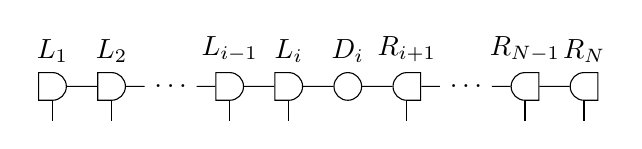
\begin{tikzpicture}[baseline=-0.25em]
        \node[ltensor, label=\(L_1\)]     (A1) at (0, 0) {};
        \node[ltensor, label=\(L_2\)]     (A2) at (0.75, 0) {};
        \node[notensor]                   (A3) at (1.5, 0) {\(\ldots\)};
        \node[ltensor, label=\(L_{i-1}\)] (A4) at (2.25, 0) {};
        \node[ltensor, label=\(L_{i}\)]   (A5) at (3, 0) {};
        \node[ctensor, label=\(D_i\)]     (D) at (3.75, 0) {};
        \node[rtensor, label=\(R_{i+1}\)] (A6) at (4.5, 0) {};
        \node[notensor]                   (A7) at (5.25, 0) {\(\ldots\)};
        \node[rtensor, label=\(R_{N-1}\)] (A8) at (6, 0) {};
        \node[rtensor, label=\(R_N\)]     (A9) at (6.75, 0) {};
        \draw (A1.south) -- +(0, -0.25);
        \draw (A2.south) -- +(0, -0.25);
        \draw (A4.south) -- +(0, -0.25);
        \draw (A5.south) -- +(0, -0.25);
        \draw (A6.south) -- +(0, -0.25);
        \draw (A8.south) -- +(0, -0.25);
        \draw (A9.south) -- +(0, -0.25);
        \draw (A1) -- (A2) -- (A3) -- (A4) -- (A5) -- (D) -- (A6) -- (A7) -- (A8) -- (A9);
    \end{tikzpicture}
    .
\end{equation}
Unitary gauge transformation:
\begin{equation}
    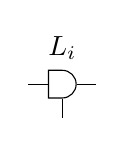
\begin{tikzpicture}[baseline=-0.25em]
        \node[ltensor, label=\(L_i\)] (A1) at (1, 0) {};
        \draw (A1.south) -- +(0, -0.25);
        \draw (A1.west) -- +(-0.25, 0);
        \draw (A1.east) -- +(0.25, 0);
    \end{tikzpicture}
    \rightarrow
    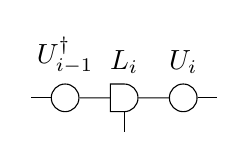
\begin{tikzpicture}[baseline=-0.25em]
        \node[ctensor, label=\(U_{i-1}^\dag\)] (G0inv) at (0.25, 0) {};
        \node[ltensor, label=\(L_i\)] (A1) at (1, 0) {};
        \node[ctensor, label=\(U_i\)] (G1) at (1.75, 0) {};
        \draw (A1.south) -- +(0, -0.25);
        \draw (G0inv.west) -- +(-0.25, 0);
        \draw (G1.east) -- +(0.25, 0);
        \draw (G0inv) -- (A1) -- (G1);
    \end{tikzpicture}
    .
\end{equation}
Expectation value:
\begin{equation}
    \braket{\Psi|O_i|\Psi} =
    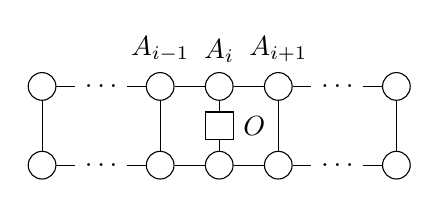
\begin{tikzpicture}[baseline=-0.25em]
        \node[atensor]                    (A1) at (0, 0.5) {};
        \node[notensor]                   (A2) at (0.75, 0.5) {\(\ldots\)};
        \node[atensor, label=\(A_{i-1}\)] (A3) at (1.5, 0.5) {};
        \node[atensor, label=\(A_i\)]     (A4) at (2.25, 0.5) {};
        \node[atensor, label=\(A_{i+1}\)] (A5) at (3, 0.5) {};
        \node[notensor]                   (A6) at (3.75, 0.5) {\(\ldots\)};
        \node[atensor]                    (A7) at (4.5, 0.5) {};
        \node[atensor]                    (A1conj) at (0, -0.5) {};
        \node[notensor]                   (A2conj) at (0.75, -0.5) {\(\ldots\)};
        \node[atensor]                    (A3conj) at (1.5, -0.5) {};
        \node[atensor]                    (A4conj) at (2.25, -0.5) {};
        \node[atensor]                    (A5conj) at (3, -0.5) {};
        \node[notensor]                   (A6conj) at (3.75, -0.5) {\(\ldots\)};
        \node[atensor]                    (A7conj) at (4.5, -0.5) {};
        \node[wtensor, label=right:\(O\)] (O) at (2.25, 0) {};
        \draw (A1) -- (A1conj);
        \draw (A3) -- (A3conj);
        \draw (A4) -- (O) -- (A4conj);
        \draw (A5) -- (A5conj);
        \draw (A7) -- (A7conj);
        \draw (A1) -- (A2) -- (A3) -- (A4) -- (A5) -- (A6) -- (A7);
        \draw (A1conj) -- (A2conj) -- (A3conj) -- (A4conj) -- (A5conj) -- (A6conj) -- (A7conj);
    \end{tikzpicture}
    .
\end{equation}
\begin{equation}
    \braket{\Psi|O_i|\Psi} =
    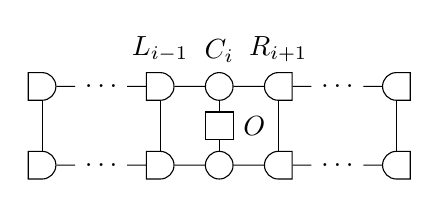
\begin{tikzpicture}[baseline=-0.25em]
        \node[ltensor]                    (A1) at (0, 0.5) {};
        \node[notensor]                   (A2) at (0.75, 0.5) {\(\ldots\)};
        \node[ltensor, label=\(L_{i-1}\)] (A3) at (1.5, 0.5) {};
        \node[atensor, label=\(C_i\)]     (A4) at (2.25, 0.5) {};
        \node[rtensor, label=\(R_{i+1}\)] (A5) at (3, 0.5) {};
        \node[notensor]                   (A6) at (3.75, 0.5) {\(\ldots\)};
        \node[rtensor]                    (A7) at (4.5, 0.5) {};
        \node[ltensor]                    (A1conj) at (0, -0.5) {};
        \node[notensor]                   (A2conj) at (0.75, -0.5) {\(\ldots\)};
        \node[ltensor]                    (A3conj) at (1.5, -0.5) {};
        \node[atensor]                    (A4conj) at (2.25, -0.5) {};
        \node[rtensor]                    (A5conj) at (3, -0.5) {};
        \node[notensor]                   (A6conj) at (3.75, -0.5) {\(\ldots\)};
        \node[rtensor]                    (A7conj) at (4.5, -0.5) {};
        \node[wtensor, label=right:\(O\)] (O) at (2.25, 0) {};
        \draw (A1) -- (A1conj);
        \draw (A3) -- (A3conj);
        \draw (A4) -- (O) -- (A4conj);
        \draw (A5) -- (A5conj);
        \draw (A7) -- (A7conj);
        \draw (A1) -- (A2) -- (A3) -- (A4) -- (A5) -- (A6) -- (A7);
        \draw (A1conj) -- (A2conj) -- (A3conj) -- (A4conj) -- (A5conj) -- (A6conj) -- (A7conj);
    \end{tikzpicture}
    =
    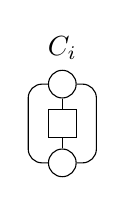
\begin{tikzpicture}[baseline=-0.25em]
        \node[atensor, label=\(C_i\)] (A4) at (2.25, 0.5) {};
        \node[atensor]                (A4conj) at (2.25, -0.5) {};
        \node[wtensor]                (O) at (2.25, 0) {};
        \draw (A4) -- (O) -- (A4conj);
        \draw[rounded corners=5pt] (A4.west) -- +(-0.25, 0) -- +(-0.25, -1) -- (A4conj.west);
        \draw[rounded corners=5pt] (A4.east) -- +(0.25, 0) -- +(0.25, -1) -- (A4conj.east);
    \end{tikzpicture}
    .
\end{equation}
Multi-site expectation value:
\begin{equation}
    \braket{\Psi|O|\Psi} =
    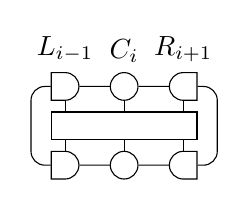
\begin{tikzpicture}[baseline=-0.25em]
        \node[ltensor, label=\(L_{i-1}\)]  (A3) at (1.5, 0.5) {};
        \node[atensor, label=\(C_i\)]      (A4) at (2.25, 0.5) {};
        \node[rtensor, label=\(R_{i+1}\)]  (A5) at (3, 0.5) {};
        \node[ltensor]                     (A3conj) at (1.5, -0.5) {};
        \node[atensor]                     (A4conj) at (2.25, -0.5) {};
        \node[rtensor]                     (A5conj) at (3, -0.5) {};
        \node[wtensor, minimum width=52.667pt] (O) at (2.25, 0) {};
        \draw (A3) -- (O.north -| A3);
        \draw (A3conj) -- (O.south -| A3conj);
        \draw (A4) -- (O.north -| A4);
        \draw (A4conj) -- (O.south -| A4conj);
        \draw (A5) -- (O.north -| A5);
        \draw (A5conj) -- (O.south -| A5conj);
        \draw (A3) -- (A4) -- (A5);
        \draw (A3conj) -- (A4conj) -- (A5conj);
        \draw[rounded corners=5pt] (A3.west) -- +(-0.25, 0) -- +(-0.25, -1) -- (A3conj.west);
        \draw[rounded corners=5pt] (A5.east) -- +(0.25, 0) -- +(0.25, -1) -- (A5conj.east);
    \end{tikzpicture}
    .
\end{equation}
MPO:
\begin{equation}
    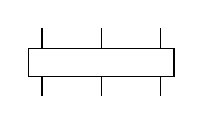
\begin{tikzpicture}[baseline=-0.25em]
        \node[wtensor, minimum width=52.667pt] (O) at (2.25, 0) {};
        \coordinate (A3) at (1.5, 0.5) {};
        \coordinate (A4) at (2.25, 0.5) {};
        \coordinate (A5) at (3, 0.5) {};
        \draw (O.north -| A3) -- +(0, 0.25);
        \draw (O.south -| A3) -- +(0, -0.25);
        \draw (O.north -| A4) -- +(0, 0.25);
        \draw (O.south -| A4) -- +(0, -0.25);
        \draw (O.north -| A5) -- +(0, 0.25);
        \draw (O.south -| A5) -- +(0, -0.25);
    \end{tikzpicture}
    =
    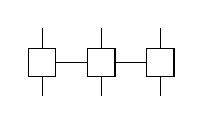
\begin{tikzpicture}[baseline=-0.25em]
        \node[wtensor] (W3) at (1.5, 0) {};
        \node[wtensor] (W4) at (2.25, 0) {};
        \node[wtensor] (W5) at (3, 0) {};
        \draw (W3.north) -- +(0, 0.25);
        \draw (W3.south) -- +(0, -0.25);
        \draw (W4.north) -- +(0, 0.25);
        \draw (W4.south) -- +(0, -0.25);
        \draw (W5.north) -- +(0, 0.25);
        \draw (W5.south) -- +(0, -0.25);
        \draw (W3) -- (W4) -- (W5);
    \end{tikzpicture}
    .
\end{equation}
MPO expectation value:
\begin{equation}
    \braket{\Psi|H|\Psi} =
    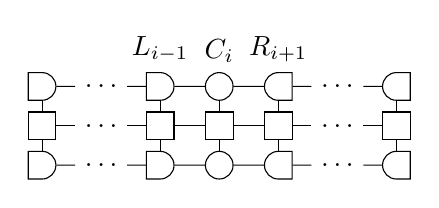
\begin{tikzpicture}[baseline=-0.25em]
        \node[ltensor]                    (A1) at (0, 0.5) {};
        \node[notensor]                   (A2) at (0.75, 0.5) {\(\ldots\)};
        \node[ltensor, label=\(L_{i-1}\)] (A3) at (1.5, 0.5) {};
        \node[atensor, label=\(C_i\)]     (A4) at (2.25, 0.5) {};
        \node[rtensor, label=\(R_{i+1}\)] (A5) at (3, 0.5) {};
        \node[notensor]                   (A6) at (3.75, 0.5) {\(\ldots\)};
        \node[rtensor]                    (A7) at (4.5, 0.5) {};
        \node[ltensor]                    (A1conj) at (0, -0.5) {};
        \node[notensor]                   (A2conj) at (0.75, -0.5) {\(\ldots\)};
        \node[ltensor]                    (A3conj) at (1.5, -0.5) {};
        \node[atensor]                    (A4conj) at (2.25, -0.5) {};
        \node[rtensor]                    (A5conj) at (3, -0.5) {};
        \node[notensor]                   (A6conj) at (3.75, -0.5) {\(\ldots\)};
        \node[rtensor]                    (A7conj) at (4.5, -0.5) {};
        \node[wtensor]                    (W1) at (0, 0) {};
        \node[notensor]                   (W2) at (0.75, 0) {\(\ldots\)};
        \node[wtensor]                    (W3) at (1.5, 0) {};
        \node[wtensor]                    (W4) at (2.25, 0) {};
        \node[wtensor]                    (W5) at (3, 0) {};
        \node[notensor]                   (W6) at (3.75, 0) {\(\ldots\)};
        \node[wtensor]                    (W7) at (4.5, 0) {};
        \draw (A1) -- (W1) -- (A1conj);
        \draw (A3) -- (W3) -- (A3conj);
        \draw (A4) -- (W4) -- (A4conj);
        \draw (A5) -- (W5) -- (A5conj);
        \draw (A7) -- (W7) -- (A7conj);
        \draw (A1) -- (A2) -- (A3) -- (A4) -- (A5) -- (A6) -- (A7);
        \draw (W1) -- (W2) -- (W3) -- (W4) -- (W5) -- (W6) -- (W7);
        \draw (A1conj) -- (A2conj) -- (A3conj) -- (A4conj) -- (A5conj) -- (A6conj) -- (A7conj);
    \end{tikzpicture}
    =
    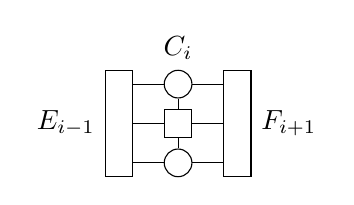
\begin{tikzpicture}[baseline=-0.25em]
        \node[atensor, label=\(C_i\)]           (A4) at (0, 0.5) {};
        \node[atensor]                          (A4conj) at (0, -0.5) {};
        \node[wtensor]                          (W4) at (0, 0) {};
        \node[etensor, label=left:\(E_{i-1}\)]  (E) at (-0.75, 0) {};
        \node[etensor, label=right:\(F_{i+1}\)] (F) at (0.75, 0) {};
        \draw (A4) -- (W4) -- (A4conj);
        \draw (E) -- (W4) -- (F);
        \draw (A4) -- (E.east |- A4);
        \draw (A4conj) -- (E.east |- A4conj);
        \draw (A4) -- (F.west |- A4);
        \draw (A4conj) -- (F.west |- A4conj);
    \end{tikzpicture}
    =
    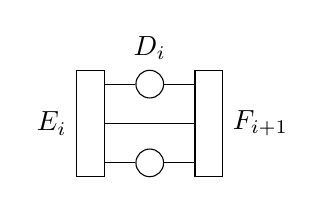
\begin{tikzpicture}[baseline=-0.25em]
        \node[ctensor, label=\(D_i\)]           (A4) at (0, 0.5) {};
        \node[ctensor]                          (A4conj) at (0, -0.5) {};
        \node[etensor, label=left:\(E_i\)]      (E) at (-0.75, 0) {};
        \node[etensor, label=right:\(F_{i+1}\)] (F) at (0.75, 0) {};
        \draw (E) -- (F);
        \draw (A4) -- (E.east |- A4);
        \draw (A4conj) -- (E.east |- A4conj);
        \draw (A4) -- (F.west |- A4);
        \draw (A4conj) -- (F.west |- A4conj);
    \end{tikzpicture}
    .
\end{equation}
Environment tensors:
\begin{equation}
    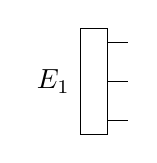
\begin{tikzpicture}[baseline=-0.25em]
        \coordinate (A4) at (0, 0.5) {};
        \coordinate (A4conj) at (0, -0.5) {};
        \node[etensor, label=left:\(E_1\)] (E) at (-0.75, 0) {};
        \draw (E.east) -- +(0.25, 0);
        \draw (E.east |- A4) -- +(0.25, 0);
        \draw (E.east |- A4conj) -- +(0.25, 0);
    \end{tikzpicture}
    \equiv
    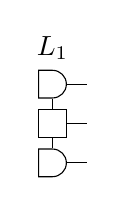
\begin{tikzpicture}[baseline=-0.25em]
        \node[ltensor, label=\(L_1\)] (A1) at (0, 0.5) {};
        \node[ltensor]                (A1conj) at (0, -0.5) {};
        \node[wtensor]                (W1) at (0, 0) {};
        \draw (A1.east) -- +(0.25, 0);
        \draw (A1conj.east) -- +(0.25, 0);
        \draw (W1.east) -- +(0.25, 0);
        \draw (A1) -- (W1) -- (A1conj);
    \end{tikzpicture}
    ,\qquad
    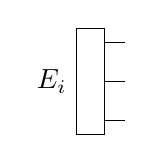
\begin{tikzpicture}[baseline=-0.25em]
        \coordinate (A4) at (0, 0.5) {};
        \coordinate (A4conj) at (0, -0.5) {};
        \node[etensor, label=left:\(E_i\)] (E) at (-0.75, 0) {};
        \draw (E.east) -- +(0.25, 0);
        \draw (E.east |- A4) -- +(0.25, 0);
        \draw (E.east |- A4conj) -- +(0.25, 0);
    \end{tikzpicture}
    \equiv
    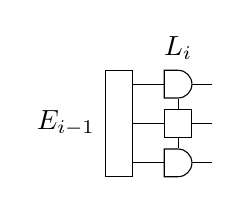
\begin{tikzpicture}[baseline=-0.25em]
        \node[ltensor, label=\(L_i\)]          (A1) at (0, 0.5) {};
        \node[ltensor]                         (A1conj) at (0, -0.5) {};
        \node[wtensor]                         (W1) at (0, 0) {};
        \node[etensor, label=left:\(E_{i-1}\)] (E) at (-0.75, 0) {};
        \draw (A1.east) -- +(0.25, 0);
        \draw (A1conj.east) -- +(0.25, 0);
        \draw (W1.east) -- +(0.25, 0);
        \draw (A1) -- (W1) -- (A1conj);
        \draw (E) -- (W1);
        \draw (A1) -- (E.east |- A1);
        \draw (A1conj) -- (E.east |- A1conj);
    \end{tikzpicture}
    .
\end{equation}
\begin{equation}
    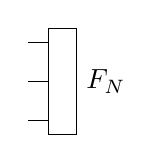
\begin{tikzpicture}[baseline=-0.25em]
        \coordinate (A4) at (0, 0.5) {};
        \coordinate (A4conj) at (0, -0.5) {};
        \node[etensor, label=right:\(F_N\)] (F) at (0.75, 0) {};
        \draw (F.west) -- +(-0.25, 0);
        \draw (F.west|- A4) -- +(-0.25, 0);
        \draw (F.west |- A4conj) -- +(-0.25, 0);
    \end{tikzpicture}
    \equiv
    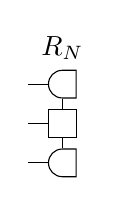
\begin{tikzpicture}[baseline=-0.25em]
        \node[rtensor, label=\(R_N\)] (A1) at (0, 0.5) {};
        \node[rtensor]                (A1conj) at (0, -0.5) {};
        \node[wtensor]                (W1) at (0, 0) {};
        \draw (A1.west) -- +(-0.25, 0);
        \draw (A1conj.west) -- +(-0.25, 0);
        \draw (W1.west) -- +(-0.25, 0);
        \draw (A1) -- (W1) -- (A1conj);
    \end{tikzpicture}
    ,\qquad
    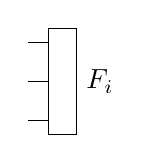
\begin{tikzpicture}[baseline=-0.25em]
        \coordinate (A4) at (0, 0.5) {};
        \coordinate (A4conj) at (0, -0.5) {};
        \node[etensor, label=right:\(F_i\)] (F) at (0.75, 0) {};
        \draw (F.west) -- +(-0.25, 0);
        \draw (F.west|- A4) -- +(-0.25, 0);
        \draw (F.west |- A4conj) -- +(-0.25, 0);
    \end{tikzpicture}
    \equiv
    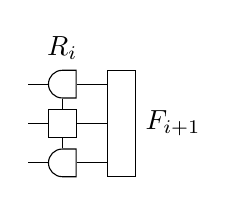
\begin{tikzpicture}[baseline=-0.25em]
        \node[rtensor, label=\(R_i\)]           (A1) at (0, 0.5) {};
        \node[rtensor]                          (A1conj) at (0, -0.5) {};
        \node[wtensor]                          (W1) at (0, 0) {};
        \node[etensor, label=right:\(F_{i+1}\)] (F) at (0.75, 0) {};
        \draw (A1.west) -- +(-0.25, 0);
        \draw (A1conj.west) -- +(-0.25, 0);
        \draw (W1.west) -- +(-0.25, 0);
        \draw (A1) -- (W1) -- (A1conj);
        \draw (W1) -- (F);
        \draw (A1) -- (F.west |- A1);
        \draw (A1conj) -- (F.west |- A1conj);
    \end{tikzpicture}
    .
\end{equation}
iMPS:
\begin{equation}
    \ket{\Psi} =
    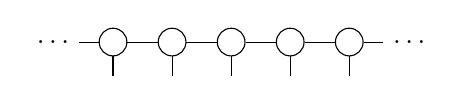
\begin{tikzpicture}[baseline=-0.25em]
        \node[atensor] (A1) at (0, 0) {};
        \node[atensor] (A2) at (0.75, 0) {};
        \node[atensor] (A3) at (1.5, 0) {};
        \node[atensor] (A4) at (2.25, 0) {};
        \node[atensor] (A5) at (3, 0) {};
        \draw (A1.south) -- +(0, -0.25);
        \draw (A2.south) -- +(0, -0.25);
        \draw (A3.south) -- +(0, -0.25);
        \draw (A4.south) -- +(0, -0.25);
        \draw (A5.south) -- +(0, -0.25);
        \draw (A1) -- (A2) -- (A3) -- (A4) -- (A5);
        \draw (A1.west) -- +(-0.25, 0) node[left] {\(\ldots\)};
        \draw (A5.east) -- +(0.25, 0) node[right] {\(\ldots\)};
    \end{tikzpicture}
    .
\end{equation}
Transfer matrix:
\begin{equation}
    T =
    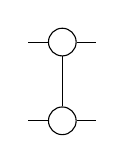
\begin{tikzpicture}[baseline=-0.25em]
        \node[atensor] (A1) at (0, 0.5) {};
        \node[atensor] (A1conj) at (0, -0.5) {};
        \draw (A1) -- (A1conj);
        \draw (A1.west) -- +(-0.25, 0);
        \draw (A1.east) -- +(0.25, 0);
        \draw (A1conj.west) -- +(-0.25, 0);
        \draw (A1conj.east) -- +(0.25, 0);
    \end{tikzpicture}
    .
\end{equation}
MPS norm:
\begin{equation}
    \braket{\Psi|\Psi} =
    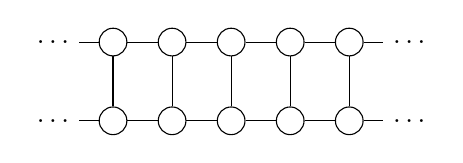
\begin{tikzpicture}[baseline=-0.25em]
        \node[atensor] (A1) at (0, 0.5) {};
        \node[atensor] (A2) at (0.75, 0.5) {};
        \node[atensor] (A3) at (1.5, 0.5) {};
        \node[atensor] (A4) at (2.25, 0.5) {};
        \node[atensor] (A5) at (3, 0.5) {};
        \node[atensor] (A1conj) at (0, -0.5) {};
        \node[atensor] (A2conj) at (0.75, -0.5) {};
        \node[atensor] (A3conj) at (1.5, -0.5) {};
        \node[atensor] (A4conj) at (2.25, -0.5) {};
        \node[atensor] (A5conj) at (3, -0.5) {};
        \draw (A1) -- (A1conj);
        \draw (A2) -- (A2conj);
        \draw (A3) -- (A3conj);
        \draw (A4) -- (A4conj);
        \draw (A5) -- (A5conj);
        \draw (A1) -- (A2) -- (A3) -- (A4) -- (A5);
        \draw (A1conj) -- (A2conj) -- (A3conj) -- (A4conj) -- (A5conj);
        \draw (A1.west) -- +(-0.25, 0) node[left] {\(\ldots\)};
        \draw (A5.east) -- +(0.25, 0) node[right] {\(\ldots\)};
        \draw (A1conj.west) -- +(-0.25, 0) node[left] {\(\ldots\)};
        \draw (A5conj.east) -- +(0.25, 0) node[right] {\(\ldots\)};
    \end{tikzpicture}
    .
\end{equation}
Left-orthogonal form:
\begin{equation}
    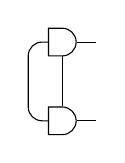
\begin{tikzpicture}[baseline=-0.25em]
        \node[ltensor] (A1) at (0, 0.5) {};
        \node[ltensor] (A1conj) at (0, -0.5) {};
        \draw (A1.south) -- (A1conj.north);
        \draw[rounded corners=5pt] (A1.west) -- +(-0.25, 0) -- +(-0.25, -1) -- (A1conj.west);
        \draw (A1.east) -- +(0.25, 0);
        \draw (A1conj.east) -- +(0.25, 0);
    \end{tikzpicture}
    =
    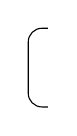
\begin{tikzpicture}[baseline=-0.25em]
        \draw[rounded corners=5pt] (0, 0.5) -- +(-0.25, 0) -- +(-0.25, -1) -- +(0, -1);
    \end{tikzpicture}
    ,
    \qquad
    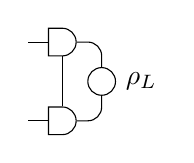
\begin{tikzpicture}[baseline=-0.25em]
        \node[ltensor] (A1) at (0, 0.5) {};
        \node[ltensor] (A1conj) at (0, -0.5) {};
        \node[ctensor, label=right:\(\rho_L\)] (rho) at (0.5, 0) {};
        \draw (A1.south) -- (A1conj.north);
        \draw[rounded corners=5pt] (A1.east) -- (A1.east -| rho.north) -- (rho) -- (rho.south |- A1conj.east) -- (A1conj.east);
        \draw (A1.west) -- +(-0.25, 0);
        \draw (A1conj.west) -- +(-0.25, 0);
    \end{tikzpicture}
    =
    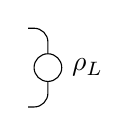
\begin{tikzpicture}[baseline=-0.25em]
        \coordinate (A1) at (0, 0.5) {};
        \coordinate (A1conj) at (0, -0.5) {};
        \node[ctensor, label=right:\(\rho_L\)] (rho) at (0.5, 0) {};
        \draw[rounded corners=5pt] (rho.north) -- (rho.north |- A1.east) -- +(-0.25, 0);
        \draw[rounded corners=5pt] (rho.south) -- (rho.south |- A1conj.east) -- +(-0.25, 0);
    \end{tikzpicture}
    .
\end{equation}
Right-orthogonal form:
\begin{equation}
    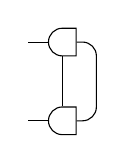
\begin{tikzpicture}[baseline=-0.25em]
        \node[rtensor] (A1) at (0, 0.5) {};
        \node[rtensor] (A1conj) at (0, -0.5) {};
        \draw (A1.south) -- (A1conj.north);
        \draw[rounded corners=5pt] (A1.east) -- +(0.25, 0) -- +(0.25, -1) -- (A1conj.east);
        \draw (A1.west) -- +(-0.25, 0);
        \draw (A1conj.west) -- +(-0.25, 0);
    \end{tikzpicture}
    =
    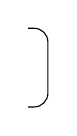
\begin{tikzpicture}[baseline=-0.25em]
        \draw[rounded corners=5pt] (0, 0.5) -- +(0.25, 0) -- +(0.25, -1) -- +(0, -1);
    \end{tikzpicture}
    ,
    \qquad
    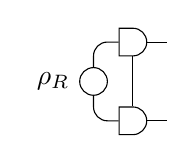
\begin{tikzpicture}[baseline=-0.25em]
        \node[ltensor] (A1) at (0, 0.5) {};
        \node[ltensor] (A1conj) at (0, -0.5) {};
        \node[ctensor, label=left:\(\rho_R\)] (rho) at (-0.5, 0) {};
        \draw (A1.south) -- (A1conj.north);
        \draw[rounded corners=5pt] (A1.west) -- (A1.west -| rho.north) -- (rho) -- (rho.south |- A1conj.west) -- (A1conj.west);
        \draw (A1.east) -- +(0.25, 0);
        \draw (A1conj.east) -- +(0.25, 0);
    \end{tikzpicture}
    =
    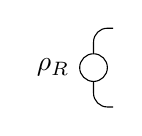
\begin{tikzpicture}[baseline=-0.25em]
        \coordinate (A1) at (0, 0.5) {};
        \coordinate (A1conj) at (0, -0.5) {};
        \node[ctensor, label=left:\(\rho_R\)] (rho) at (-0.5, 0) {};
        \draw[rounded corners=5pt] (rho.north) -- (rho.north |- A1.west) -- +(0.25, 0);
        \draw[rounded corners=5pt] (rho.south) -- (rho.south |- A1conj.west) -- +(0.25, 0);
    \end{tikzpicture}
    .
\end{equation}
Mixed-canonical form:
\begin{align}
    \ket{\Psi} &=
    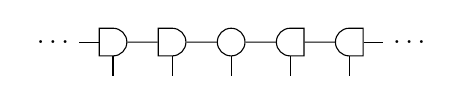
\begin{tikzpicture}[baseline=-0.25em]
        \node[ltensor] (A1) at (0, 0) {};
        \node[ltensor] (A2) at (0.75, 0) {};
        \node[atensor] (A3) at (1.5, 0) {};
        \node[rtensor] (A4) at (2.25, 0) {};
        \node[rtensor] (A5) at (3, 0) {};
        \draw (A1.south) -- +(0, -0.25);
        \draw (A2.south) -- +(0, -0.25);
        \draw (A3.south) -- +(0, -0.25);
        \draw (A4.south) -- +(0, -0.25);
        \draw (A5.south) -- +(0, -0.25);
        \draw (A1) -- (A2) -- (A3) -- (A4) -- (A5);
        \draw (A1.west) -- +(-0.25, 0) node[left] {\(\ldots\)};
        \draw (A5.east) -- +(0.25, 0) node[right] {\(\ldots\)};
    \end{tikzpicture}
    \\
    &=
    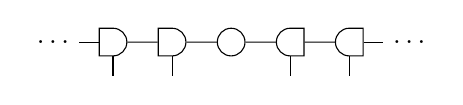
\begin{tikzpicture}[baseline=-0.25em]
        \node[ltensor] (A1) at (0, 0) {};
        \node[ltensor] (A2) at (0.75, 0) {};
        \node[ctensor] (A3) at (1.5, 0) {};
        \node[rtensor] (A4) at (2.25, 0) {};
        \node[rtensor] (A5) at (3, 0) {};
        \draw (A1.south) -- +(0, -0.25);
        \draw (A2.south) -- +(0, -0.25);
        \draw (A4.south) -- +(0, -0.25);
        \draw (A5.south) -- +(0, -0.25);
        \draw (A1) -- (A2) -- (A3) -- (A4) -- (A5);
        \draw (A1.west) -- +(-0.25, 0) node[left] {\(\ldots\)};
        \draw (A5.east) -- +(0.25, 0) node[right] {\(\ldots\)};
    \end{tikzpicture}
    .
\end{align}
iMPS expectation value:
\begin{equation}
    \braket{\Psi|O_i|\Psi} =
    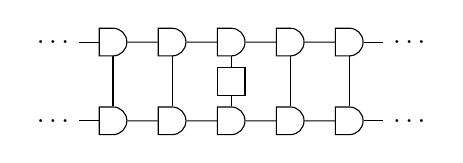
\begin{tikzpicture}[baseline=-0.25em]
        \node[ltensor] (A1) at (0, 0.5) {};
        \node[ltensor] (A2) at (0.75, 0.5) {};
        \node[ltensor] (A3) at (1.5, 0.5) {};
        \node[ltensor] (A4) at (2.25, 0.5) {};
        \node[ltensor] (A5) at (3, 0.5) {};
        \node[ltensor] (A1conj) at (0, -0.5) {};
        \node[ltensor] (A2conj) at (0.75, -0.5) {};
        \node[ltensor] (A3conj) at (1.5, -0.5) {};
        \node[ltensor] (A4conj) at (2.25, -0.5) {};
        \node[ltensor] (A5conj) at (3, -0.5) {};
        \node[wtensor] (O) at (1.5, 0) {};
        \draw (A1) -- (A1conj);
        \draw (A2) -- (A2conj);
        \draw (A3) -- (O) -- (A3conj);
        \draw (A4) -- (A4conj);
        \draw (A5) -- (A5conj);
        \draw (A1) -- (A2) -- (A3) -- (A4) -- (A5);
        \draw (A1conj) -- (A2conj) -- (A3conj) -- (A4conj) -- (A5conj);
        \draw (A1.west) -- +(-0.25, 0) node[left] {\(\ldots\)};
        \draw (A5.east) -- +(0.25, 0) node[right] {\(\ldots\)};
        \draw (A1conj.west) -- +(-0.25, 0) node[left] {\(\ldots\)};
        \draw (A5conj.east) -- +(0.25, 0) node[right] {\(\ldots\)};
    \end{tikzpicture}
    =
    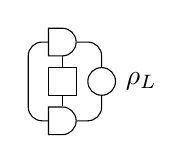
\begin{tikzpicture}[baseline=-0.25em]
        \node[ltensor] (A4) at (2.25, 0.5) {};
        \node[ltensor] (A4conj) at (2.25, -0.5) {};
        \node[wtensor] (O) at (2.25, 0) {};
        \node[ctensor, label=right:\(\rho_L\)] (rho) at (2.75, 0) {};
        \draw (A4) -- (O) -- (A4conj);
        \draw[rounded corners=5pt] (A4.west) -- +(-0.25, 0) -- +(-0.25, -1) -- (A4conj.west);
        \draw[rounded corners=5pt] (A4.east) -- (A4.east -| rho.north) -- (rho) -- (rho.south |- A4conj.east) -- (A4conj.east);
    \end{tikzpicture}
    .
\end{equation}
\begin{equation}
    \braket{\Psi|O_i|\Psi} =
    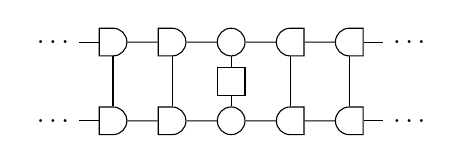
\begin{tikzpicture}[baseline=-0.25em]
        \node[ltensor] (A1) at (0, 0.5) {};
        \node[ltensor] (A2) at (0.75, 0.5) {};
        \node[atensor] (A3) at (1.5, 0.5) {};
        \node[rtensor] (A4) at (2.25, 0.5) {};
        \node[rtensor] (A5) at (3, 0.5) {};
        \node[ltensor] (A1conj) at (0, -0.5) {};
        \node[ltensor] (A2conj) at (0.75, -0.5) {};
        \node[atensor] (A3conj) at (1.5, -0.5) {};
        \node[rtensor] (A4conj) at (2.25, -0.5) {};
        \node[rtensor] (A5conj) at (3, -0.5) {};
        \node[wtensor] (O) at (1.5, 0) {};
        \draw (A1) -- (A1conj);
        \draw (A2) -- (A2conj);
        \draw (A3) -- (O) -- (A3conj);
        \draw (A4) -- (A4conj);
        \draw (A5) -- (A5conj);
        \draw (A1) -- (A2) -- (A3) -- (A4) -- (A5);
        \draw (A1conj) -- (A2conj) -- (A3conj) -- (A4conj) -- (A5conj);
        \draw (A1.west) -- +(-0.25, 0) node[left] {\(\ldots\)};
        \draw (A5.east) -- +(0.25, 0) node[right] {\(\ldots\)};
        \draw (A1conj.west) -- +(-0.25, 0) node[left] {\(\ldots\)};
        \draw (A5conj.east) -- +(0.25, 0) node[right] {\(\ldots\)};
    \end{tikzpicture}
    =
    \begin{tikzpicture}[baseline=-0.25em]
        \node[atensor] (A4) at (2.25, 0.5) {};
        \node[atensor] (A4conj) at (2.25, -0.5) {};
        \node[wtensor] (O) at (2.25, 0) {};
        \draw (A4) -- (O) -- (A4conj);
        \draw[rounded corners=5pt] (A4.west) -- +(-0.25, 0) -- +(-0.25, -1) -- (A4conj.west);
        \draw[rounded corners=5pt] (A4.east) -- +(0.25, 0) -- +(0.25, -1) -- (A4conj.east);
    \end{tikzpicture}
    .
\end{equation}
Environment tensor recursion relation:
\begin{equation}
    \begin{tikzpicture}[baseline=-0.25em]
        \coordinate (A4) at (0, 0.5) {};
        \coordinate (A4conj) at (0, -0.5) {};
        \node[etensor, label=left:\(E(n+1)\)] (E) at (-0.75, 0) {};
        \draw (E.east) -- +(0.25, 0) node[right] {\(\alpha\)};
        \draw (E.east |- A4) -- +(0.25, 0);
        \draw (E.east |- A4conj) -- +(0.25, 0);
    \end{tikzpicture}
    =
    \begin{tikzpicture}[baseline=-0.25em]
        \node[ltensor] (A1) at (0, 0.5) {};
        \node[ltensor] (A1conj) at (0, -0.5) {};
        \node[wtensor]  (W1) at (0, 0) {};
        \node[etensor, label=left:\(E(n)\)] (E) at (-0.75, 0) {};
        \draw (A1.east) -- +(0.25, 0);
        \draw (A1conj.east) -- +(0.25, 0);
        \draw (W1.east) -- +(0.25, 0) node[right] {\(\scriptstyle\alpha\)};
        \draw (A1) -- (W1) -- (A1conj);
        \draw (E.east) -- +(0.1, 0);
        \draw (W1.west) -- +(-0.1, 0);
        \node at (-0.375, 0) {\(\scriptstyle\alpha\)};
        \draw (A1) -- (E.east |- A1);
        \draw (A1conj) -- (E.east |- A1conj);
    \end{tikzpicture}
    + \sum_{\beta<\alpha}
    \begin{tikzpicture}[baseline=-0.25em]
        \node[ltensor] (A1) at (0, 0.5) {};
        \node[ltensor] (A1conj) at (0, -0.5) {};
        \node[wtensor]  (W1) at (0, 0) {};
        \node[etensor, label=left:\(E(n)\)] (E) at (-0.75, 0) {};
        \draw (A1.east) -- +(0.25, 0);
        \draw (A1conj.east) -- +(0.25, 0);
        \draw (W1.east) -- +(0.25, 0) node[right] {\(\scriptstyle\alpha\)};
        \draw (A1) -- (W1) -- (A1conj);
        \draw (E.east) -- +(0.1, 0);
        \draw (W1.west) -- +(-0.1, 0);
        \node at (-0.375, 0) {\(\scriptstyle\beta\)};
        \draw (A1) -- (E.east |- A1);
        \draw (A1conj) -- (E.east |- A1conj);
    \end{tikzpicture}
    .
\end{equation}
\end{document}
